\section{Результаты вычислительных методов}

\subsection{Характеристики вычислительной системы для проведения экспериментов}

Спецификация системы: 

 Polus - параллельная вычислительная система, состоящая из 5 вычислительных узлов. (на первый вычислительный узел возложены функции frontend узла)
 
\noindent Основные характеристики каждого узла:
\begin{itemize}
    \item 2 десятиядерных процессора IBM POWER8 (каждое ядро имеет 8 потоков) всего 160 потоков
    \item Общая оперативная память 256 Гбайт (в узле 5 оперативная память 1024 Гбайт) с ЕСС контролем
    \item 2 х 1 ТБ 2.5” 7K RPM SATA HDD
    \item 2 x NVIDIA Tesla P100 GPU, 16Gb, NVLink
    \item 1 порт 100 ГБ/сек
\end{itemize}

\noindent Производительность кластера (Tflop/s): 55,84 (пиковая), 40,39 (Linpack) \\

\subsection{Описание экспериментов}
Рассмотрим теперь вопрос об эффективности алгоритма. Для этого напомним, что
каждый параллельный алгоритм оценивается по двум параметрам – ускорению $S_p$ и
эффективности $E_p$ , которые определяются по формулам:
$$S_p = {{t_1} \over {t_p}},$$ $$E_p = {S_p \over p} * 100\%$$
где $t_1$ - время решения исходной задачи на одном процессоре, $t_p$ - время
решения исходной задачи по параллельному алгоритму на p процессорах.

Для оценки работы алгоритма с точки зрения качества реконструкции поверхности были проведены следующие эксперименты:\\ 
Были взяты полигональные модели разные по сложности формы начиная от обычного куба и заканчивая морским ежом(см. рис. \ref{fig:polygonal models}). Все модели были предварительно нормированы следующим образом: сдвинуты центром масс к началу координат, все вершины модели были отмасштабированы так, что максимальное отклонение от начала координат было менее 1. Данные полигональные модели впоследствии будем называть эталонными.\\
С полигональных моделей были взяты 200000 случайных точек(см. рис. \ref{fig:point cloud models}).\\ 
Облако точек с эталонной модели зашумлялось аддитивным гауссовым шумом с различным среднеквадратичным отклонением. Данное облако точек впоследствии использовались в качестве входных данных алгоритма MLS.\\
К зашумленному облаку точек применялся алгоритм MLS с различным параметром $\bold{R}$. Восстановленная алгоритмом MLS поверхность представленная набором точек сравнивалась с эталонной моделью.
Были посчитаны среднее отклонение восстановленной поверхности от эталонной модели, а также среднеквадратичное отклонение (Таблицы \ref{table:1}, \ref{table:2}, \ref{table:3}, \ref{table:4}, \ref{table:5}, \ref{table:6}). По результатам исследований алгоритм MLS хорошо справляется с зашумленными данными, но для достижения оптимальных результатов нужно тщательно подбирать параметр радиуса алгоритма. Это особенно касается моделей сложной формы. Слишком маленький радиус может вести к потере данных ввиду невозможности найти локальную плоскость, а слишком большой ведет к размытию резких контуров поверхности.

\begin{figure}[h]
  \centering
    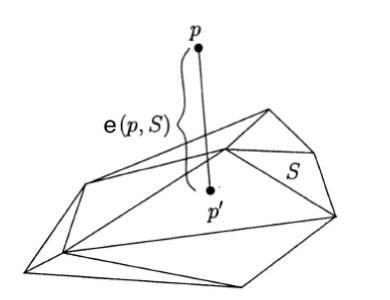
\includegraphics[width=0.8\textwidth]{images/distance.jpg}
  \caption{Отклонение $e_i(p, S)$ — это расстояние между точкой и поверхностью S. Точка $p^{'}$ — ближайшая точка к поверхности S.}
\end{figure}

\clearpage
\subsection{Картинки, таблицы, графики}

\begin{table}[h]
\begin{tabular}{|c|c|c|c|c|}
    \hline
    $R$ & Число MPI-процессов & Время работы (с) & Ускорение & Эффективность \\
    \hline
    0.0008 & 1 & 601.91  &  1  &  100.0 \\
    0.0008 & 2 & 356.632  &  1.69  &  84.39 \\
    0.0008 & 4 & 210.948  &  2.85  &  71.33 \\
    0.0008 & 8 & 124.986  &  4.82  &  60.2 \\
    0.0008 & 16 & 73.742  &  8.16  &  51.01 \\
    0.0008 & 32 & 43.434  &  13.86  &  43.31 \\
    \hline
    0.0012 &  1  &  1070.74  &  1  &  100.0 \\
    0.0012 &  2  &  615.675  &  1.74  &  86.96 \\
    0.0012 &  4  &  342.008  &  3.13  &  78.27 \\
    0.0012 &  8  &  193.405  &  5.54  &  69.2 \\
    0.0012 &  16  &  110.338  &  9.7  &  60.65 \\
    0.0012 &  32  &  63.003  &  17.0  &  53.11 \\
    \hline
    0.0016 &  1  &  1959.78  &  1  &  100.0 \\
    0.0016 &  2  &  1093.557  &  1.79  &  89.61 \\
    0.0016 &  4  &  579.585  &  3.38  &  84.53 \\
    0.0016 &  8  &  310.948  &  6.3  &  78.78 \\
    0.0016 &  16  &  168.845  &  11.61  &  72.54 \\
    0.0016 &  32  &  90.501  &  21.65  &  67.67 \\
    \hline
\end{tabular}
\caption{Результаты запуска программы для различных значений параметра R. На вход подавалось облако из 25000000 точек.}
\label{table:1}
\end{table}

На графиках представлены измерения для различных значений параметра R при изменении количества MPI процессов. Из графика эффективности видно, что при большем радиусе, эффективность падает медленнее. Это связано с увеличением количества локальных вычислений при тех же затратах на коммуникации между процессами.


\begin{figure}[h]
    \centering
    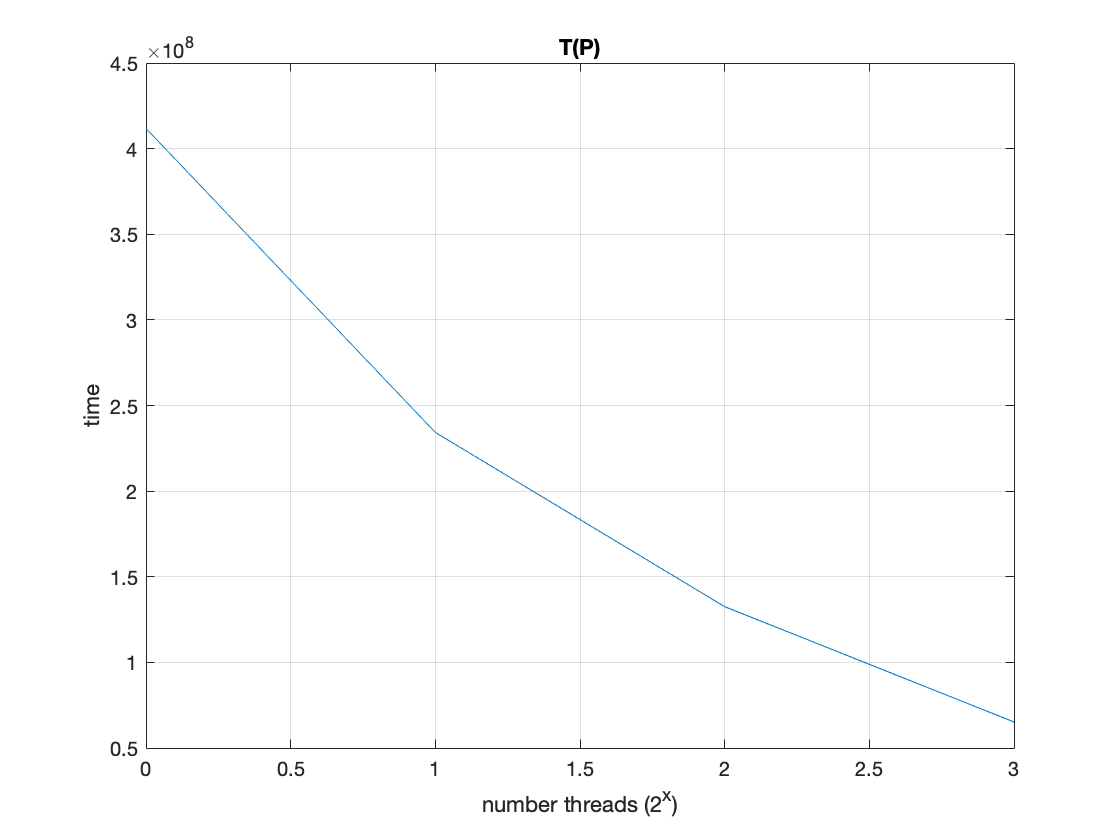
\includegraphics[scale=0.6]{T(P).png}
    \caption{Время работы (c) на n процессах n = 1...32}
    \label{fig:mesh1}
\end{figure}

\begin{figure}[h]
    \centering
    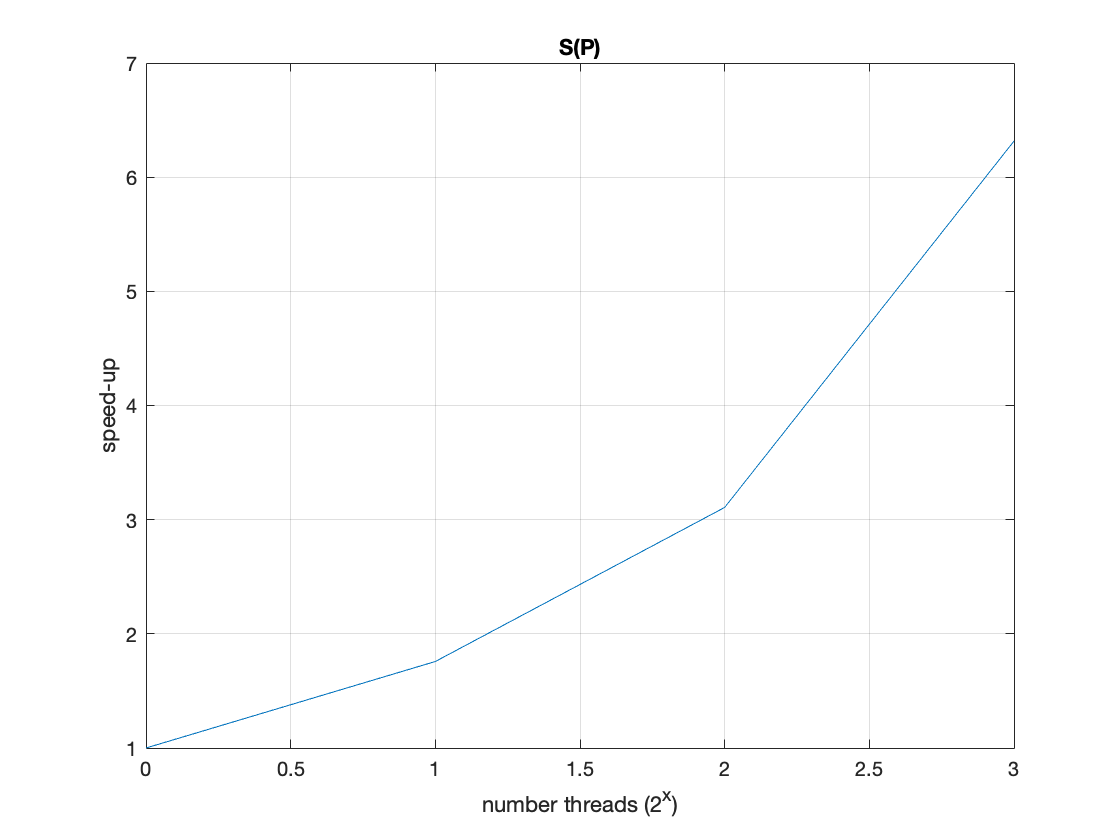
\includegraphics[scale=0.6]{S(P).png}
    \caption{Ускорение}
    \label{fig:mesh1}
\end{figure}

\begin{figure}[h]
    \centering
    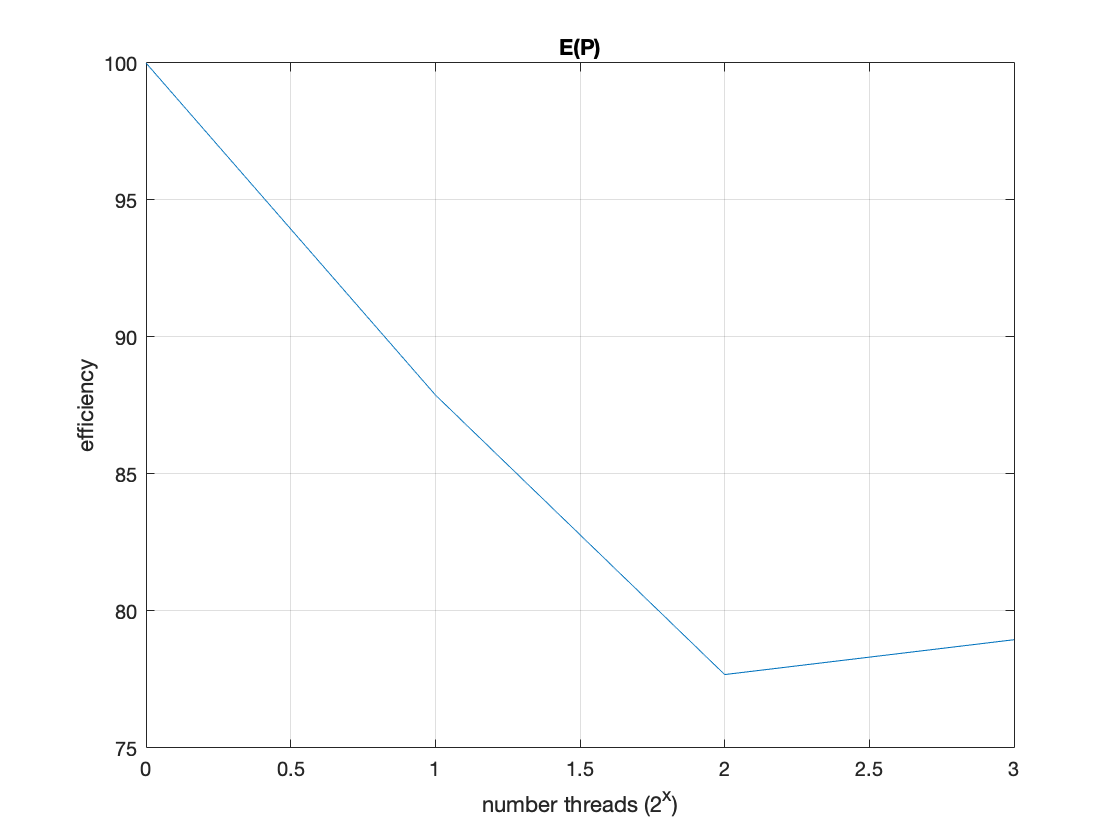
\includegraphics[scale=0.6]{E(P).png}
    \caption{Эффективность}
    \label{fig:mesh1}
\end{figure}

\begin{table}[h]
\begin{tabular}{|c|c|c|c|c|c|}
    \hline
    $R$ & Число MPI-процессов & Число OpenMP-нитей & Время работы (с)  \\
    \hline\hline
    0.0008 &  1  & 1  &  601.91 \\
    0.0008 &  2  & 1  &  356.632 \\
    0.0008 &  4  & 1  &  210.948 \\
    0.0008 &  8  & 1  &  124.986 \\
    \hline
    0.0008 &  1  & 2  &  340.348 \\
    0.0008 &  2  & 2  &  201.095 \\
    0.0008 &  4  & 2  &  117.203 \\
    0.0008 &  8  & 2  &  68.377 \\
    \hline
    0.0008 &  1  & 4  &  183.182 \\
    0.0008 &  2  & 4  &  108.107 \\
    0.0008 &  4  & 4  &  63.591 \\
    0.0008 &  8  & 4  &  37.494 \\
    \hline\hline
    0.0012 &  1  & 1  &  1070.74 \\
    0.0012 &  2  & 1  &  615.675 \\
    0.0012 &  4  & 1  &  342.008 \\
    0.0012 &  8  & 1  &  193.405 \\
    \hline
    0.0012 &  1  & 2  &  602.795 \\
    0.0012 &  2  & 2  &  340.879 \\
    0.0012 &  4  & 2  &  187.004 \\
    0.0012 &  8  & 2  &  104.702 \\
    \hline
    0.0012 &  1  & 4  &  310.09 \\
    0.0012 &  2  & 4  &  176.728 \\
    0.0012 &  4  & 4  &  97.626 \\
    0.0012 &  8  & 4  &  55.051 \\
    \hline\hline
    0.0016 &  1  & 1  &  1959.78 \\
    0.0016 &  2  & 1  &  1093.557 \\
    0.0016 &  4  & 1  &  579.585 \\
    0.0016 &  8  & 1  &  310.948 \\
    \hline
    0.0016 &  1  & 2  &  1080.297 \\
    0.0016 &  2  & 2  &  598.387 \\
    0.0016 &  4  & 2  &  312.359 \\
    0.0016 &  8  & 2  &  166.638 \\
    \hline
    0.0016 &  1  & 4  &  558.458 \\
    0.0016 &  2  & 4  &  310.34 \\
    0.0016 &  4  & 4  &  163.279 \\
    0.0016 &  8  & 4  &  87.274 \\
    
    \hline
\end{tabular}
\caption{Результаты запуска гибридной программы для различных значений параметра R. На вход подавалось облако из 25000000 точек.}
\label{table:1}
\end{table}

\clearpage
На следующем графике представлены измерения времени работы для различных значений параметра R при изменении количества mpi процессов c применением openMP. По итогу гибридная программа оказалась эффективней чисто MPI программы.

\begin{figure}[h]
    \centering
    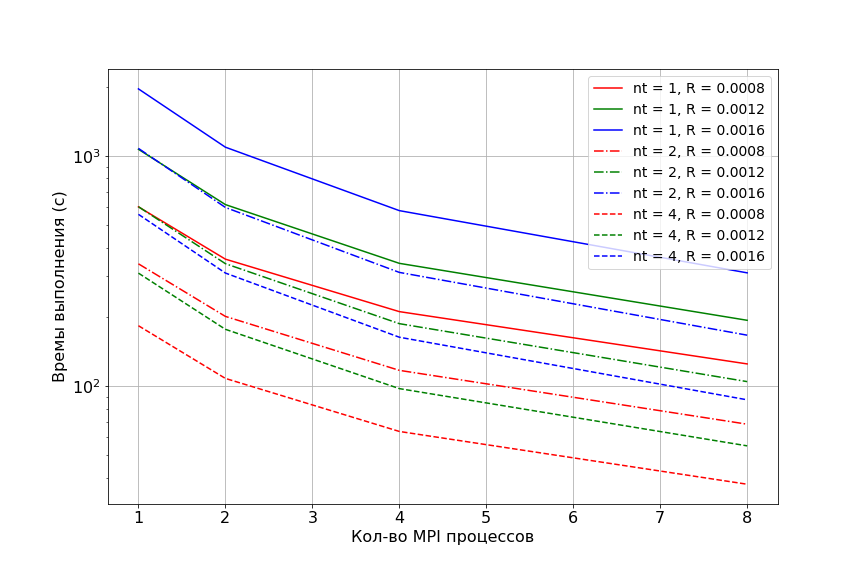
\includegraphics[scale=0.6]{images/time_1_omp.png}
    \caption{Время работы гибридной программы (MPI + OpenMP)}
    \label{fig:mesh1}
\end{figure}

\clearpage
Все полигональные модели были нормированы для того чтобы результаты на разных моделях были сравнимыми. Полигональная модель состоит из перечисления вершин и связей между ними. Для нормирования полигональной модели достаточно нормировать облако точек вершин. Связи между вершинами при этом остаются без изменений.

\begin{figure}[h]
    \centering
    \subbottom[Cube]{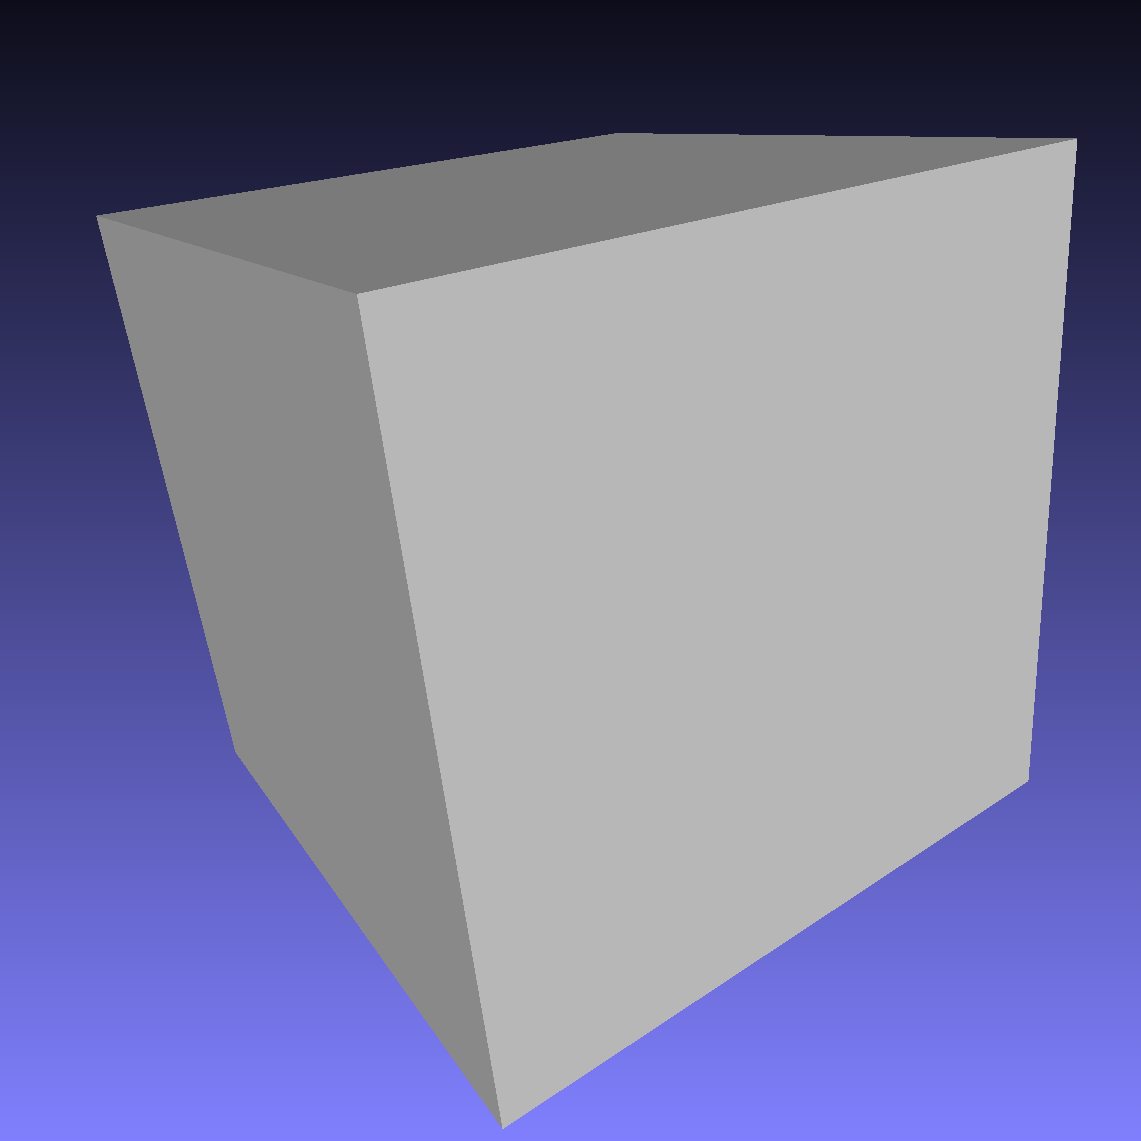
\includegraphics[width=0.32\textwidth, height=5cm]{ply/cube.png}}
    \subbottom[Woman]{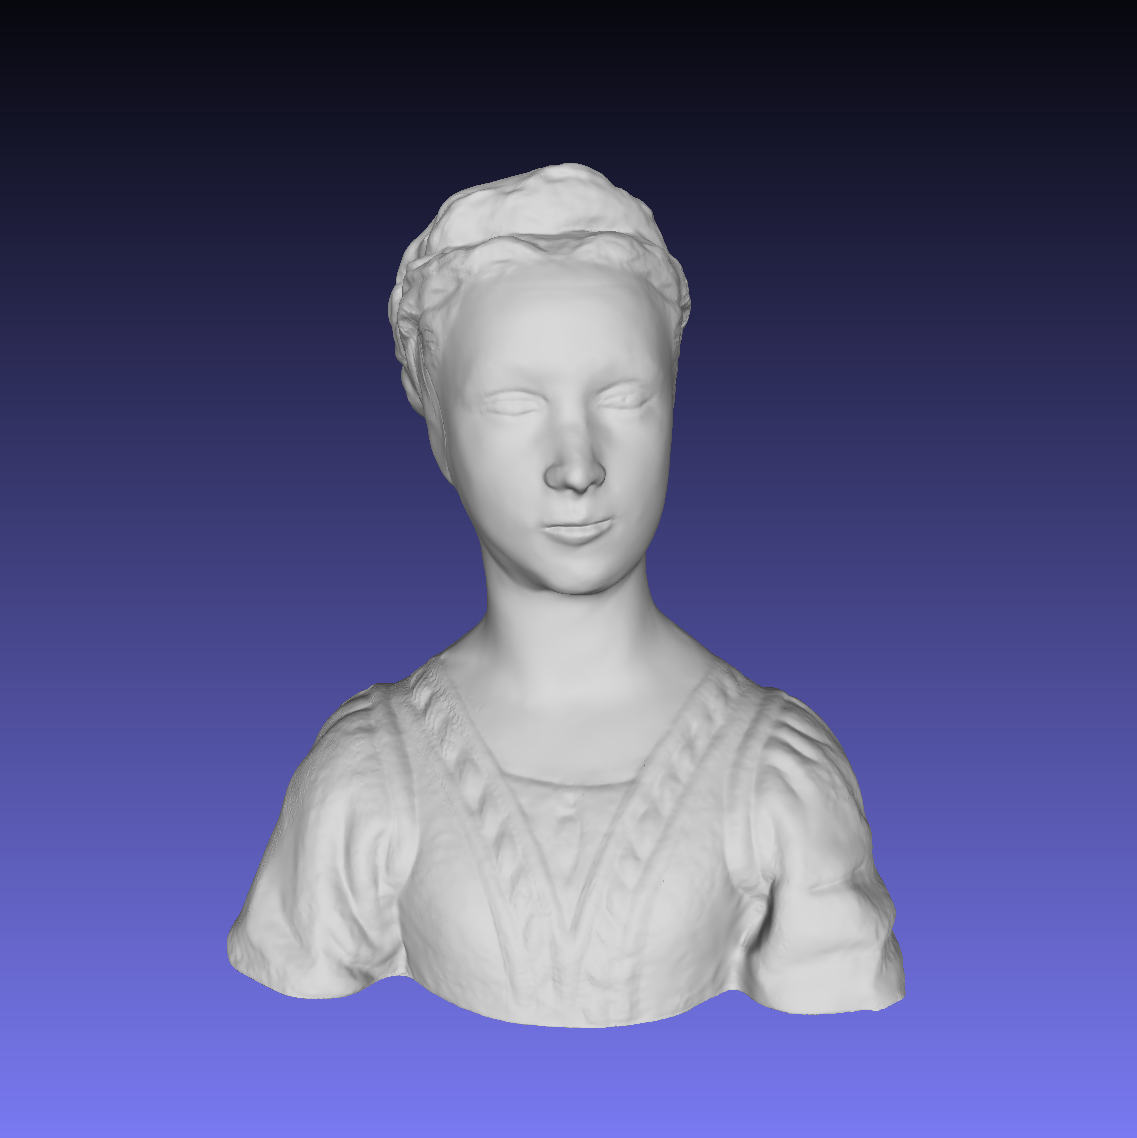
\includegraphics[width=0.32\textwidth, height=5cm]{ply/woman.png}}
    \subbottom[Elephant]{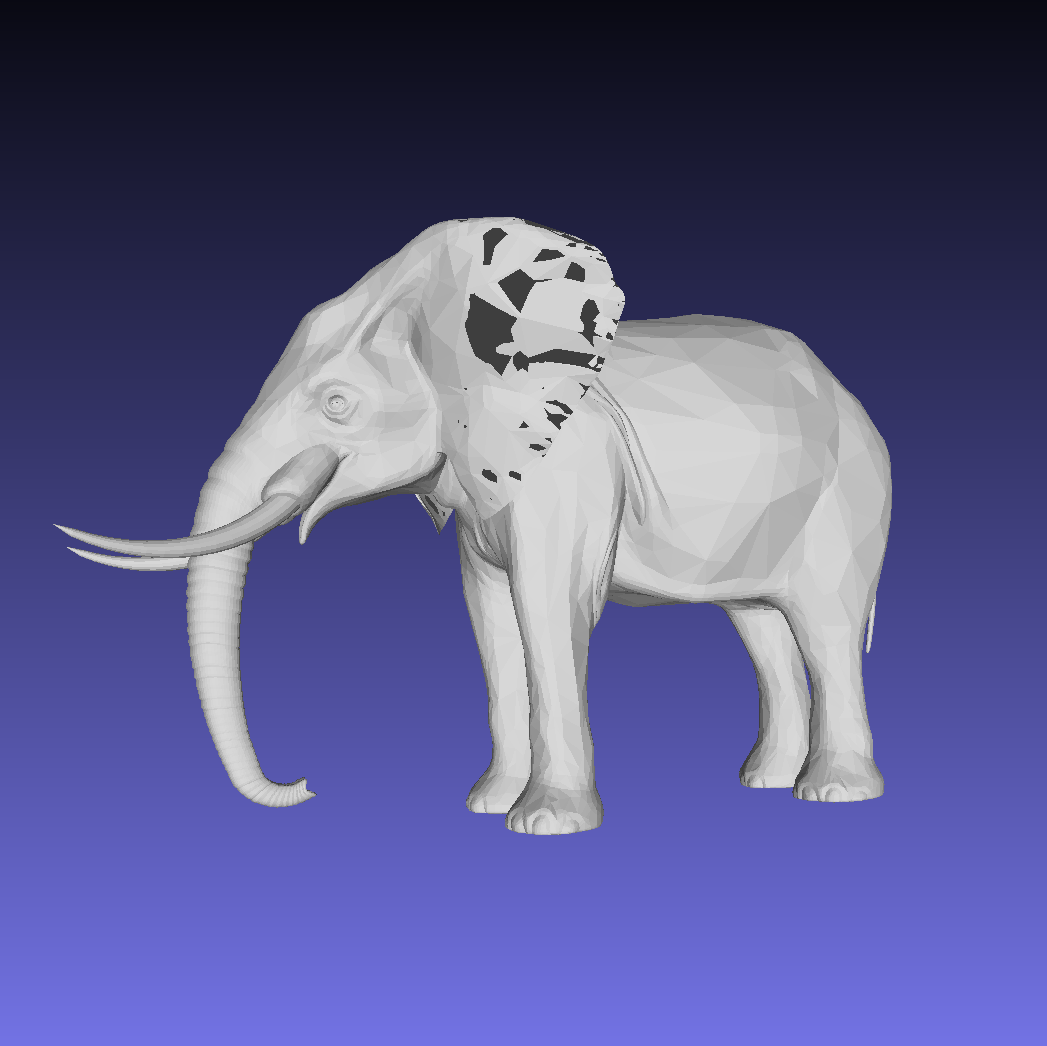
\includegraphics[width=0.32\textwidth, height=5cm]{ply/elephant.png}}
    \subbottom[Hippo]{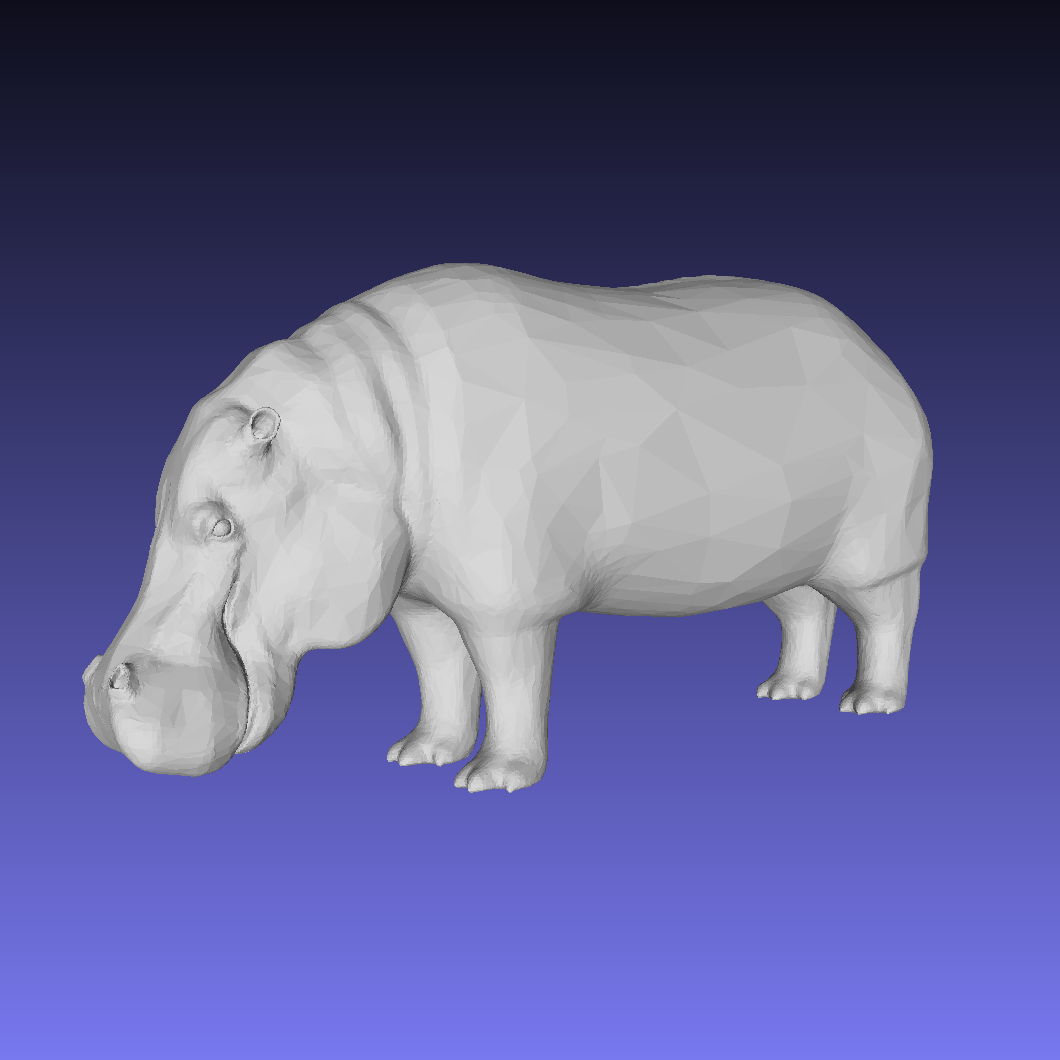
\includegraphics[width=0.32\textwidth, height=5cm]{ply/hippo.png}}
    \subbottom[Bunny]{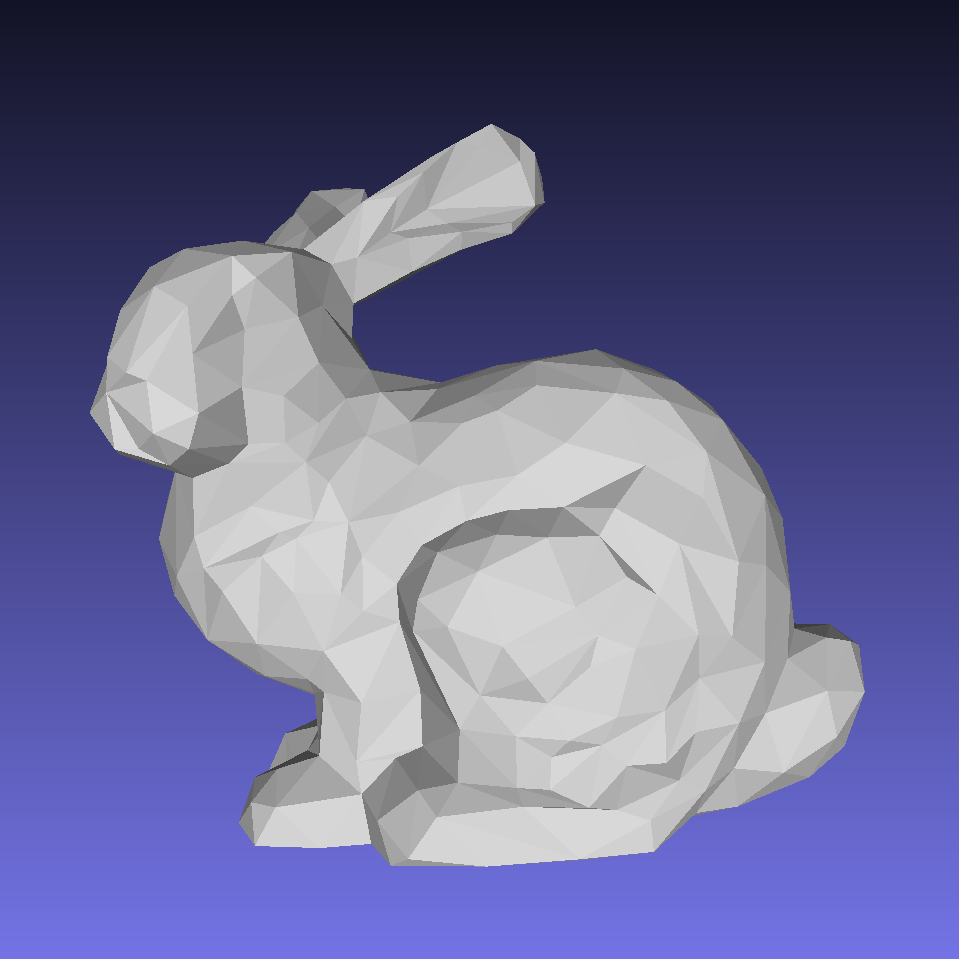
\includegraphics[width=0.32\textwidth, height=5cm]{ply/bunny.png}}
    \subbottom[Sea Urchin]{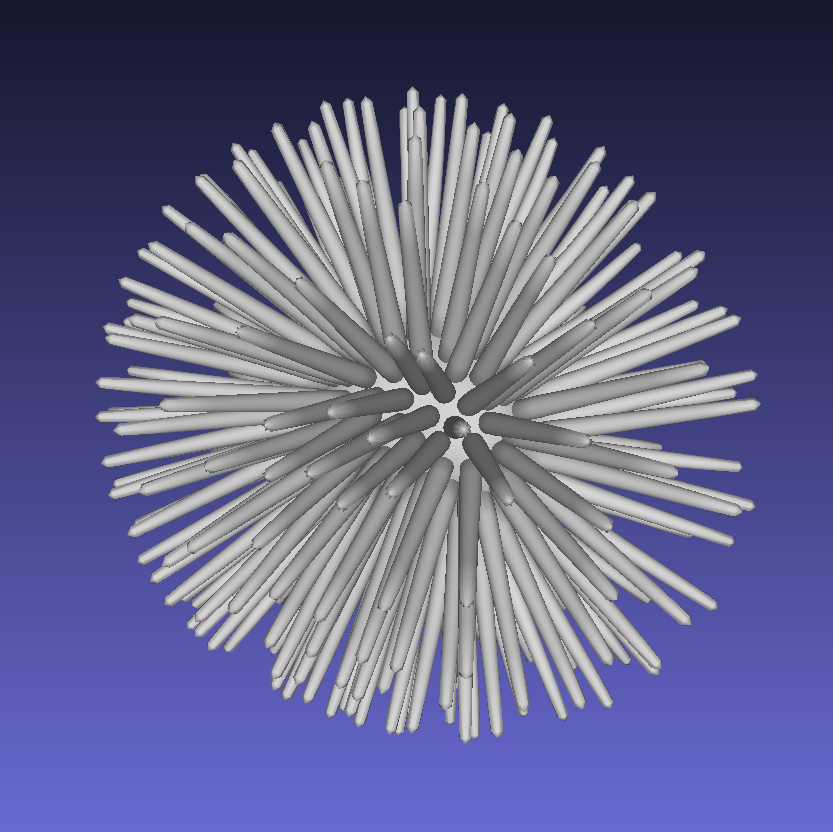
\includegraphics[width=0.32\textwidth, height=5cm]{ply/sea_urchin.png}}
    \caption{Полигональные модели для тестирования качества работы алгоритма.}
    \label{fig:polygonal models}
\end{figure}

\begin{figure}[h]
    \centering
    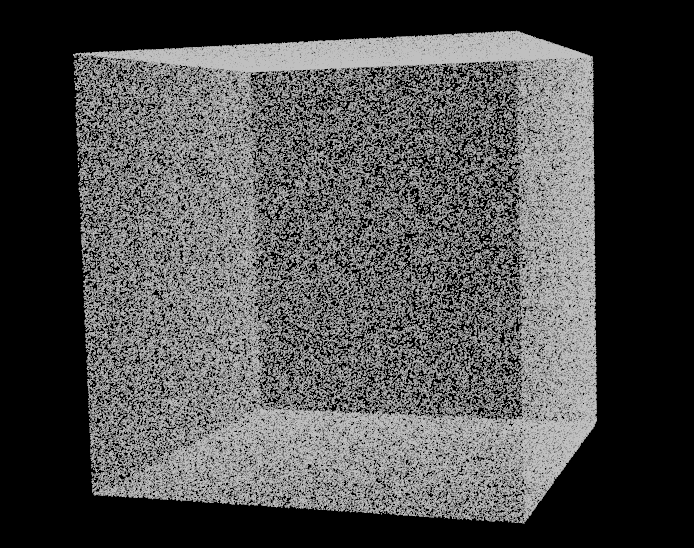
\includegraphics[width=0.32\textwidth, height=5cm]{pcd/cube.png}
    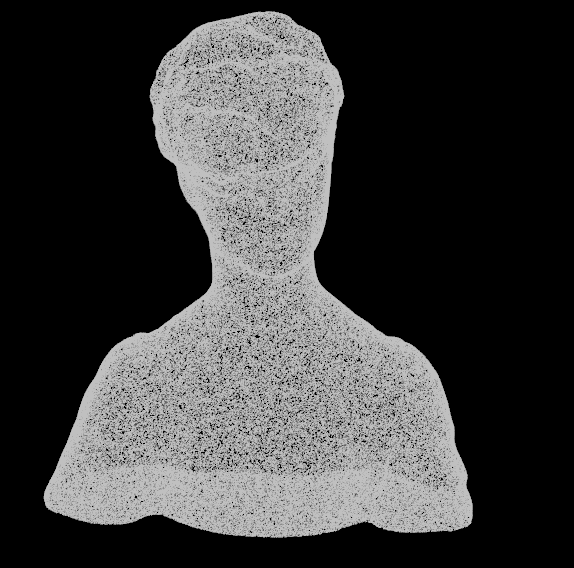
\includegraphics[width=0.32\textwidth, height=5cm]{pcd/woman.png}
    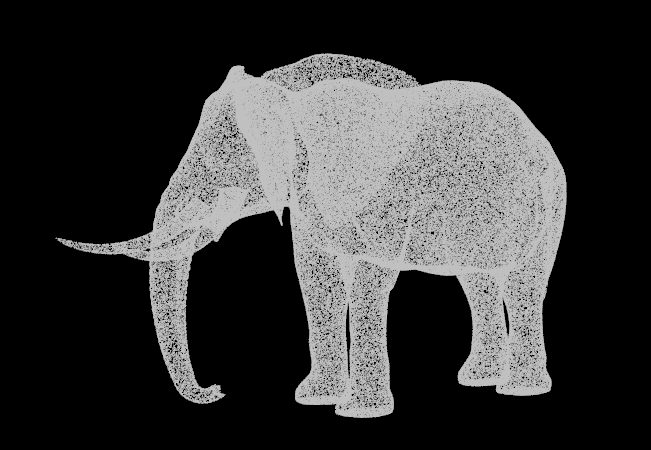
\includegraphics[width=0.32\textwidth, height=5cm]{pcd/elephant.png}
    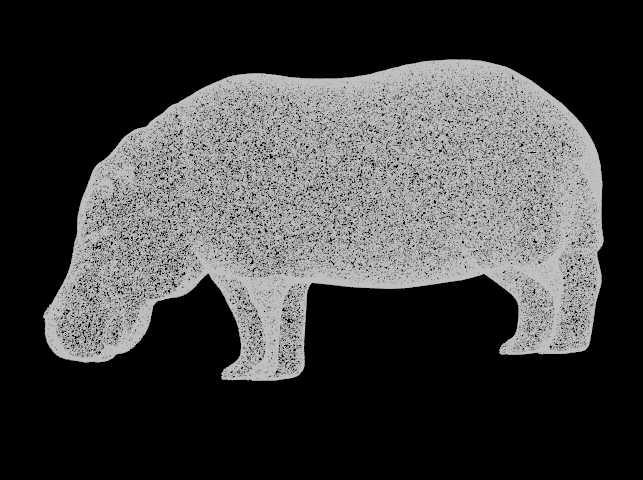
\includegraphics[width=0.32\textwidth, height=5cm]{pcd/hippo.png}
    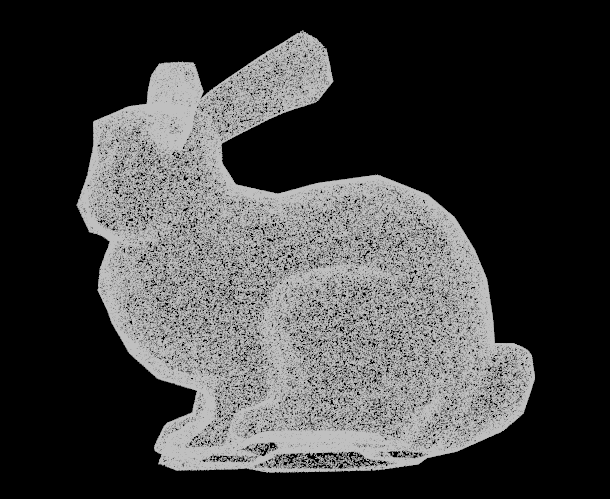
\includegraphics[width=0.32\textwidth, height=5cm]{pcd/bunny.png}
    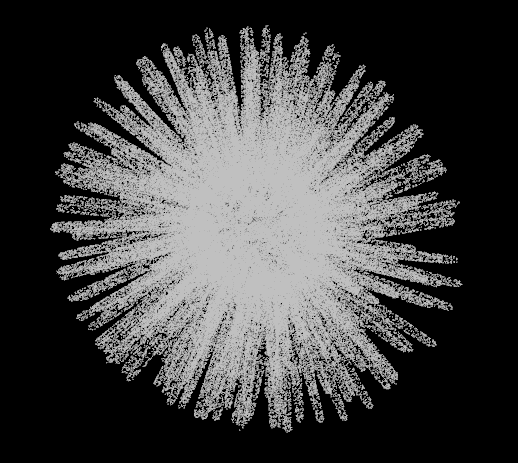
\includegraphics[width=0.32\textwidth, height=5cm]{pcd/sea_urchin.png}
    \caption{Облака точек взятые с полигональных моделей. С каждой модели взято 200000 рандомных точек.}
    \label{fig:point cloud models}
\end{figure}

\begin{figure}[h]
  \centering
  \subbottom[зашумленное облако точек с модели Bunny]{%
    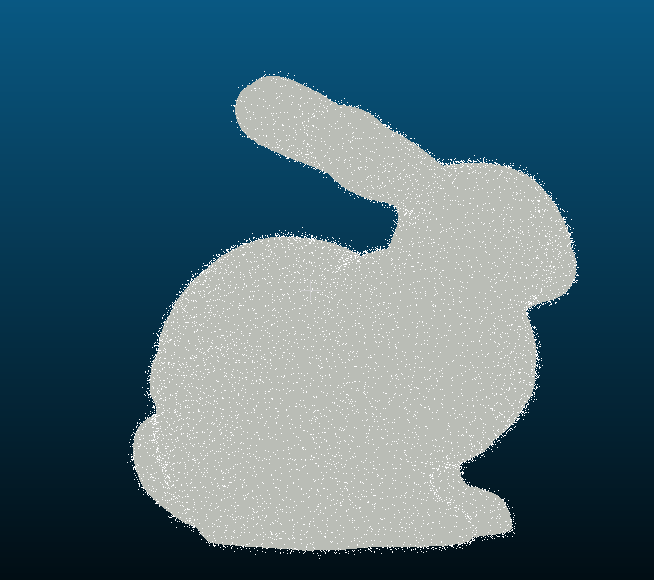
\includegraphics[width=8cm]{images/bunnyWithNoise.png}}
  \subbottom[Bunny после MLS]{%
    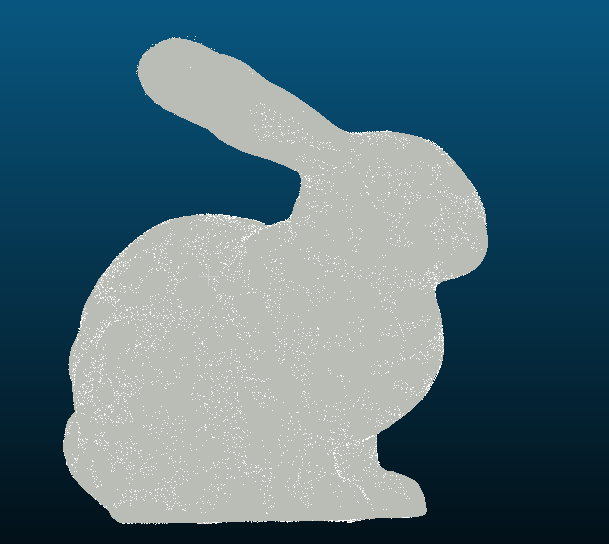
\includegraphics[width=8cm]{images/bynnyAfterMLS.png}}
  \caption{Слева зашумленное облако точек аддитивным Гауссовым шумом с $\boldsymbol{\sigma = 0.01}$ на эталонной поверхности. Справа, восстановленное облако точек методом MLS на той же эталонной поверхности.}
\end{figure}

\begin{figure}[h]
  \centering
  \subbottom[зашумленное облако точек с модели Bunny]{%
    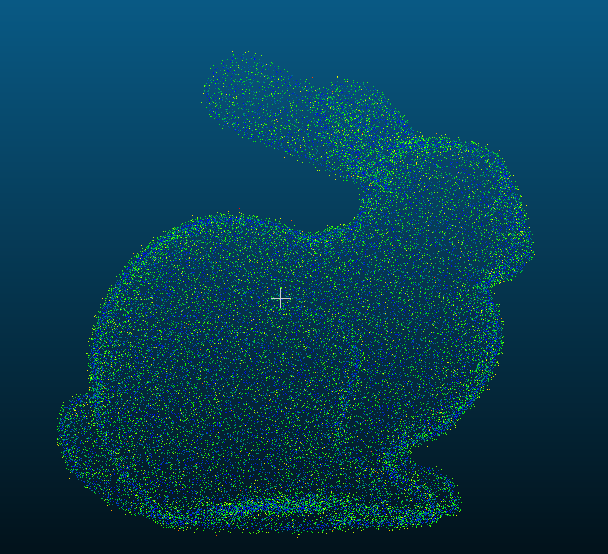
\includegraphics[width=0.49\textwidth, height=8cm]{images/bunnyWithNoiseCompare.png}}
  \subbottom[Bunny после MLS]{%
    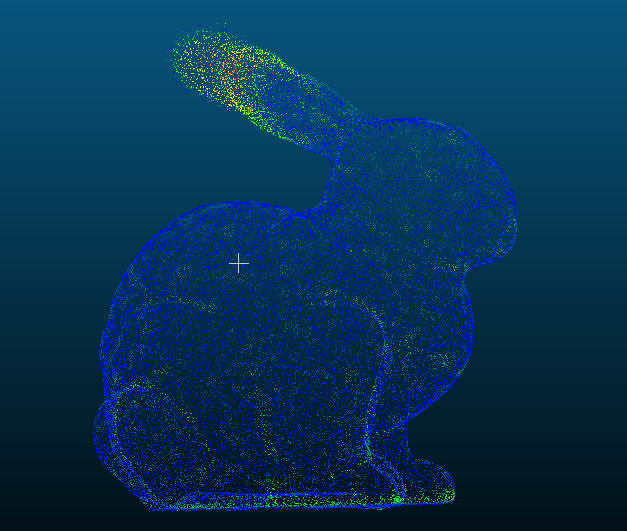
\includegraphics[width=0.49\textwidth, height=8cm]{images/bunnyAfterMLSCompare.png}}
  \caption{Слева зашумленное облако точек аддитивным Гауссовым шумом с $\boldsymbol{\sigma = 0.01}$. Справа, восстановленное облако точек методом MLS. Интенсивность цвета обозначает величину отклонения от эталонной поверхности.}
\end{figure}

В таблицах \ref{table:1}, \ref{table:2}, \ref{table:3}, \ref{table:4}, \ref{table:5}, \ref{table:6} представлены измерения для различных моделей. Цель измерений была установить положительное влияние алгоритма движущихся наименьших квадратов и  подобрать оптимальный свободный параметр (Радиус окрестности). Для всех моделей за исключением Sea Urchin (рис. \ref{fig:polygonal models} (f)) видно, что значение радиуса нужно подбирать немного больше значения среднеквадратичного отклонения шума. Это хорошая начальная оценка учитывая большой набор методов оценки распределения шума. Более точное значение параметра можно подобрать исходя из визуальной оценки используя к примеру кнопку ползунок.  Также стоит отметить для большинства моделей наличие локального минимума до значения среднеквадратичного отклонения шума. Это связано с тем, что алгоритм MLS, выбрасывает из результата те точки, для которых нашлось менее 3‑х соседей, считая такие точки выбросами. При подборе достаточно маленького радиуса это ведет к значительной потере данных.
\begin{table}[h]
\centering
\begin{tabular}{| c | c | c| c | c | c | c |}
    \hline
    применен MLS & $\sigma$ & $\bold{R}$ & ср. геом. откл. & ср. кв. откл. & min & max \\
    \hline\hline
    $\times$ & 0.005 & -- & 0.00484 & 0.00269 & 3.8e-05 & 0.0245\\
    \checkmark & 0.005 &  0.005 & 0.00372 & 0.00181 & 5.5e-05 & 0.01418\\
    \checkmark & 0.005 &  0.01 & 0.00434 & 0.00245 & 6.7e-05 & 0.01715\\
    \checkmark & 0.005 &  0.03 & \textbf{0.00248} & \textbf{0.00117} & 3.5e-05 & 0.01676\\
    \checkmark & 0.005 &  0.05 & 0.00277 & 0.00185 & 1.3e-05 & 0.02362\\
    \hline
    $\times$ & 0.01 & -- & 0.00854 & 0.00563 & 0.0001 & 0.04387\\
    \checkmark & 0.01 &  0.005 & 0.00578 & 0.00339 & 6.2e-05 & 0.02481\\
    \checkmark & 0.01 &  0.01 & 0.00741 & 0.0045 & 8.7e-05 & 0.03055\\
    \checkmark & 0.01 &  0.03 & \textbf{0.00334} & \textbf{0.002} & 9e-06 & 0.04387\\
    \checkmark & 0.01 &  0.05 & 0.00344 & 0.00226 & 6.1e-05 & 0.03942\\
    \hline
    $\times$ & 0.03 & -- & 0.02333 & 0.01722 & 0.000167 & 0.13393\\
    \checkmark & 0.03 &  0.005 & 0.01424 & 0.01001 & 0.000167 & 0.06133\\
    \checkmark & 0.03 &  0.01 & 0.01672 & 0.01168 & 0.000158 & 0.07857\\
    \checkmark & 0.03 &  0.03 & 0.02065 & 0.01572 & 0.00012 & 0.10811\\
    \checkmark & 0.03 &  0.05 & \textbf{0.01284} & \textbf{0.01116} & 8.3e-05 & 0.11659\\
    \hline
\end{tabular}

\caption{Результат работы алгоритма MLS на модели Bunny. На вход алгоритма подается облако точек с модели, зашумленное аддитивным гауссовым шумом. Сравнивается восстановленная поверхность MLS c различным параметром R с эталонной поверхностью по среднему отклонению (mean distance), среднеквадратичному отклонению (standard deviation), минимальному (min) и максимальному (max) отклонению.  $\bold{R}$ -- параметр алгоритма MLS, $\sigma$ -- среднеквадратичное отклонение аддитивного гауссового шума.}
\label{table:1}
\end{table}


\begin{table}[h]
\centering
\begin{tabular}{| c | c | c| c | c | c | c |}
    \hline
    применен MLS & $\sigma$ & $\bold{R}$ & ср. геом. откл. & ср. кв. откл. & min & max \\
    \hline\hline
    $\times$ & 0.005 & -- & 0.00528 & 0.00266 & 9e-05 & 0.0231\\
    \checkmark & 0.005 &  0.005 & 0.00394 & 0.00176 & 0.000173 & 0.01341\\
    \checkmark & 0.005 &  0.01 & 0.00481 & 0.00229 & 6.1e-05 & 0.01872\\
    \checkmark & 0.005 &  0.03 & \textbf{0.00312} & \textbf{0.00143} & 5.6e-05 & 0.01069\\
    \checkmark & 0.005 &  0.05 & 0.00323 & 0.00149 & 2.1e-05 & 0.01071\\
    \hline
    $\times$ & 0.01 & -- & 0.00896 & 0.00553 & 6.3e-05 & 0.04574\\
    \checkmark & 0.01 &  0.005 & 0.00608 & 0.00321 & 0.000239 & 0.02309\\
    \checkmark & 0.01 &  0.01 & 0.00722 & 0.00395 & 7e-05 & 0.03011\\
    \checkmark & 0.01 &  0.03 & 0.00423 & 0.00242 & 7.1e-05 & 0.04506\\
    \checkmark & 0.01 &  0.05 & \textbf{0.00363} & \textbf{0.00172} & 3e-05 & 0.01496\\
    \hline
    $\times$ & 0.03 & -- & 0.02413 & 0.0175 & 5.5e-05 & 0.13091\\
    \checkmark & 0.03 &  0.005 & 0.01506 & 0.01012 & 0.000453 & 0.06424\\
    \checkmark & 0.03 &  0.01 & 0.01603 & 0.01086 & 0.00022 & 0.08114\\
    \checkmark & 0.03 &  0.03 & 0.02172 & 0.01601 & 7.2e-05 & 0.10536\\
    \checkmark & 0.03 &  0.05 & \textbf{0.0139} & \textbf{0.0122} & 0.000107 & 0.1205\\
    \hline
\end{tabular}

\caption{Результат работы алгоритма MLS на модели Cube. На вход алгоритма подается облако точек с модели, зашумленное аддитивным гауссовым шумом. Сравнивается восстановленная поверхность MLS c различным параметром R с эталонной поверхностью по среднему отклонению (mean distance), среднеквадратичному отклонению (standard deviation), минимальному (min) и максимальному (max) отклонению.  $\bold{R}$ -- параметр алгоритма MLS, $\sigma$ -- среднеквадратичное отклонение аддитивного гауссового шума.}
\label{table:2}
\end{table}


\begin{table}[h]
\centering
\begin{tabular}{| c | c | c| c | c | c | c |}
    \hline
    применен MLS & $\sigma$ & $\bold{R}$ & ср. геом. откл. & ср. кв. откл. & min & max \\
    \hline\hline
    $\times$ & 0.005 & -- & 0.00477 & 0.00268 & 6.1e-05 & 0.02512\\
    \checkmark & 0.005 &  0.005 & 0.00368 & 0.00181 & 6.1e-05 & 0.01509\\
    \checkmark & 0.005 &  0.01 & 0.00424 & 0.00244 & 5.8e-05 & 0.0187\\
    \checkmark & 0.005 &  0.03 & \textbf{0.00265} & \textbf{0.00151} & 4.6e-05 & 0.01855\\
    \checkmark & 0.005 &  0.05 & 0.00301 & 0.00236 & 2.2e-05 & 0.02479\\
    \hline
    $\times$ & 0.01 & -- & 0.00836 & 0.00559 & 0.000109 & 0.04483\\
    \checkmark & 0.01 &  0.005 & 0.00574 & 0.00343 & 0.00012 & 0.02845\\
    \checkmark & 0.01 &  0.01 & 0.00731 & 0.0045 & 5.5e-05 & 0.03267\\
    \checkmark & 0.01 &  0.03 & \textbf{0.00347} & \textbf{0.00222} & 3.8e-05 & 0.04305\\
    \checkmark & 0.01 &  0.05 & 0.00372 & 0.00268 & 6e-05 & 0.03384\\
    \hline
    $\times$ & 0.03 & -- & 0.02264 & 0.01693 & 9.1e-05 & 0.1461\\
    \checkmark & 0.03 &  0.005 & 0.01384 & 0.01005 & 0.000269 & 0.07674\\
    \checkmark & 0.03 &  0.01 & 0.01659 & 0.01172 & 0.000124 & 0.08642\\
    \checkmark & 0.03 &  0.03 & 0.02005 & 0.01549 & 8.6e-05 & 0.10592\\
    \checkmark & 0.03 &  0.05 & \textbf{0.01301} & \textbf{0.01142} & 4.4e-05 & 0.12447\\
    \hline
\end{tabular}

\caption{Результат работы алгоритма MLS на модели Elephant. На вход алгоритма подается облако точек с модели, зашумленное аддитивным гауссовым шумом. Сравнивается восстановленная поверхность MLS c различным параметром R с эталонной поверхностью по среднему отклонению (mean distance), среднеквадратичному отклонению (standard deviation), минимальному (min) и максимальному (max) отклонению.  $\bold{R}$ -- параметр алгоритма MLS, $\sigma$ -- среднеквадратичное отклонение аддитивного гауссового шума.}
\label{table:3}
\end{table}


\begin{table}[h]
\centering
\begin{tabular}{| c | c | c| c | c | c | c |}
    \hline
    применен MLS & $\sigma$ & $\bold{R}$ & ср. геом. откл. & ср. кв. откл. & min & max \\
    \hline\hline
    $\times$ & 0.005 & -- & 0.00477 & 0.00271 & 7.4e-05 & 0.02114\\
    \checkmark & 0.005 &  0.005 & 0.00366 & 0.00181 & 5.3e-05 & 0.01381\\
    \checkmark & 0.005 &  0.01 & 0.00422 & 0.00247 & 5e-05 & 0.01848\\
    \checkmark & 0.005 &  0.03 & \textbf{0.00234} & \textbf{0.00112} & 4e-05 & 0.01742\\
    \checkmark & 0.005 &  0.05 & 0.00243 & 0.00146 & 3.6e-05 & 0.01932\\
    \hline
    $\times$ & 0.01 & -- & 0.00846 & 0.00564 & 0.000118 & 0.04645\\
    \checkmark & 0.01 &  0.005 & 0.00579 & 0.00346 & 0.000106 & 0.02456\\
    \checkmark & 0.01 &  0.01 & 0.00742 & 0.00458 & 0.000103 & 0.03196\\
    \checkmark & 0.01 &  0.03 & \textbf{0.00287} & \textbf{0.00177} & 5e-05 & 0.0449\\
    \checkmark & 0.01 &  0.05 & 0.00299 & 0.00182 & 3.9e-05 & 0.02826\\
    \hline
    $\times$ & 0.03 & -- & 0.02364 & 0.01744 & 0.000117 & 0.1768\\
    \checkmark & 0.03 &  0.005 & 0.01462 & 0.01046 & 0.000183 & 0.07097\\
    \checkmark & 0.03 &  0.01 & 0.01719 & 0.01197 & 8.8e-05 & 0.0872\\
    \checkmark & 0.03 &  0.03 & 0.0208 & 0.01593 & 3.7e-05 & 0.1069\\
    \checkmark & 0.03 &  0.05 & \textbf{0.01255} & \textbf{0.01104} & 0.0001 & 0.12441\\
    \hline
\end{tabular}

\caption{Результат работы алгоритма MLS на модели Hippo. На вход алгоритма подается облако точек с модели, зашумленное аддитивным гауссовым шумом. Сравнивается восстановленная поверхность MLS c различным параметром R с эталонной поверхностью по среднему отклонению (mean distance), среднеквадратичному отклонению (standard deviation), минимальному (min) и максимальному (max) отклонению.  $\bold{R}$ -- параметр алгоритма MLS, $\sigma$ -- среднеквадратичное отклонение аддитивного гауссового шума.}
\label{table:4}
\end{table}


\begin{table}[h]
\centering
\begin{tabular}{| c | c | c| c | c | c | c |}
    \hline
    применен MLS & $\sigma$ & $\bold{R}$ & ср. геом. откл. & ср. кв. откл. & min & max \\
    \hline\hline
    $\times$ & 0.005 & -- & 0.00624 & 0.00275 & 7.3e-05 & 0.02333\\
    \checkmark & 0.005 &  0.005 & \textbf{0.00445} & \textbf{0.00185} & 9.3e-05 & 0.0123\\
    \checkmark & 0.005 &  0.01 & 0.00526 & 0.0022 & 6.9e-05 & 0.01588\\
    \checkmark & 0.005 &  0.03 & 0.00562 & 0.00254 & 9e-05 & 0.02307\\
    \checkmark & 0.005 &  0.05 & 0.00894 & 0.00436 & 0.00017 & 0.02779\\
    \hline
    $\times$ & 0.01 & -- & 0.00956 & 0.00486 & 0.000123 & 0.04262\\
    \checkmark & 0.01 &  0.005 & \textbf{0.00683} & \textbf{0.00305} & 0.000456 & 0.01841\\
    \checkmark & 0.01 &  0.01 & 0.00752 & 0.00341 & 0.000226 & 0.02633\\
    \checkmark & 0.01 &  0.03 & 0.00863 & 0.0045 & 5.9e-05 & 0.03821\\
    \checkmark & 0.01 &  0.05 & 0.01034 & 0.00485 & 7e-05 & 0.04272\\
    \hline
    $\times$ & 0.03 & -- & 0.01812 & 0.01358 & 0.000175 & 0.1198\\
    \checkmark & 0.03 &  0.005 & \textbf{0.01033} & \textbf{0.00584} & 0.000688 & 0.05006\\
    \checkmark & 0.03 &  0.01 & 0.01103 & 0.00631 & 0.000276 & 0.05743\\
    \checkmark & 0.03 &  0.03 & 0.01652 & 0.01145 & 0.000153 & 0.09185\\
    \checkmark & 0.03 &  0.05 & 0.01624 & 0.01225 & 0.000219 & 0.09817\\
    \hline
\end{tabular}

\caption{Результат работы алгоритма MLS на модели Sea Urchin. На вход алгоритма подается облако точек с модели, зашумленное аддитивным гауссовым шумом. Сравнивается восстановленная поверхность MLS c различным параметром R с эталонной поверхностью по среднему отклонению (mean distance), среднеквадратичному отклонению (standard deviation), минимальному (min) и максимальному (max) отклонению.  $\bold{R}$ -- параметр алгоритма MLS, $\sigma$ -- среднеквадратичное отклонение аддитивного гауссового шума.}
\label{table:5}
\end{table}


\begin{table}[h]
\centering
\begin{tabular}{| c | c | c| c | c | c | c |}
    \hline
    применен MLS & $\sigma$ & $\bold{R}$ & ср. геом. откл. & ср. кв. откл. & min & max \\
    \hline\hline
    $\times$ & 0.005 & -- & 0.00486 & 0.00269 & 6.7e-05 & 0.0226\\
    \checkmark & 0.005 &  0.005 & 0.00371 & 0.00179 & 7.6e-05 & 0.01491\\
    \checkmark & 0.005 &  0.01 & 0.00437 & 0.00245 & 8.7e-05 & 0.01768\\
    \checkmark & 0.005 &  0.03 & \textbf{0.00248} & \textbf{0.00113} & 3.8e-05 & 0.01193\\
    \checkmark & 0.005 &  0.05 & 0.00256 & 0.00125 & 3.1e-05 & 0.01736\\
    \hline
    $\times$ & 0.01 & -- & 0.00856 & 0.00564 & 8.3e-05 & 0.0453\\
    \checkmark & 0.01 &  0.005 & 0.0058 & 0.00336 & 0.000122 & 0.0258\\
    \checkmark & 0.01 &  0.01 & 0.00741 & 0.00447 & 3.8e-05 & 0.03209\\
    \checkmark & 0.01 &  0.03 & 0.00329 & 0.00186 & 3e-05 & 0.04396\\
    \checkmark & 0.01 &  0.05 & \textbf{0.00313} & \textbf{0.0016} & 3.4e-05 & 0.02138\\
    \hline
    $\times$ & 0.03 & -- & 0.02359 & 0.01737 & 7.6e-05 & 0.14377\\
    \checkmark & 0.03 &  0.005 & 0.01461 & 0.01033 & 0.000214 & 0.06379\\
    \checkmark & 0.03 &  0.01 & 0.01675 & 0.01164 & 6.5e-05 & 0.09195\\
    \checkmark & 0.03 &  0.03 & 0.0208 & 0.01587 & 0.000106 & 0.10975\\
    \checkmark & 0.03 &  0.05 & \textbf{0.0124} & \textbf{0.01011} & 3.2e-05 & 0.12571\\
    \hline
\end{tabular}

\caption{Результат работы алгоритма MLS на модели Woman. На вход алгоритма подается облако точек с модели, зашумленное аддитивным гауссовым шумом. Сравнивается восстановленная поверхность MLS c различным параметром R с эталонной поверхностью по среднему отклонению (mean distance), среднеквадратичному отклонению (standard deviation), минимальному (min) и максимальному (max) отклонению.  $\bold{R}$ -- параметр алгоритма MLS, $\sigma$ -- среднеквадратичное отклонение аддитивного гауссового шума.}
\label{table:6}
\end{table}

